\chapter{Design Considerations}

\section{Similarities to MIO}
We noticed that an asynchronous syscall manager abstracting
over \texttt{io\_uring} had many similar design requirements to
the \texttt{EventManager}, namely:
\begin{enumerate}
	\item Allowing threads to submit requests,
	along with a post-completion callback

	\item Polling loop that checks for new events and
	executes callbacks if necessary; ready file descriptors
	in the case of the \texttt{EventManager}, completed
	system calls in the case of a hypothetical syscall manager

	\item One manager per Capability
\end{enumerate}

Hence, in our design of the \texttt{URingManager},
we draw heavy inspiration from the \texttt{EventManager}

\section{Tight Coupling with MIO \texttt{EventManager}}

The \texttt{network} library we used in our benchmarks was found
to be tightly coupled to the MIO \texttt{EventManager} and the threadWait API.
 
In Figure \ref{fig:networkThreadWait}, we depict code used to send the contents of a buffer
via a socket as of version 3.1.4.0. The \texttt{sendAll} function first attempts
to call \texttt{send}, a wrapper around a non-blocking send system call.
If unsuccessful with zero bytes sent, \texttt{threadWaitWrite} is called,
before re-attempting the send once the socket is ready. 

\begin{figure}[ht]
	\centering
	\lstinputlisting[language=Haskell]{figures/code/Network.hs}
	\caption[Sample code from the \texttt{network} library]{
		Sample code from the \texttt{network} library on Hackage
		version 3.1.4.0 demonstrating tight coupling
		to the \texttt{EventManager} \texttt{threadWait} API.
		Slight modifications were made from original source to
		improve understandability.
	}
	\label{fig:networkThreadWait}
\end{figure}
  
In order to have the network library take advantage of our \texttt{URingManager} backend,
we would have to write
completion-based counterparts of waiting-for-readiness logic.
We demonstrate this later in the \textbf{Example Usage} subsection of this current section.

Beyond the \texttt{network} library, the aforementioned discussion applies
more generally to any other code that depends on
\texttt{threadWait\{Read, Write\}}. Code written with the polling
paradigm is inherently incompatible with our \texttt{URingManager}’s completion paradigm.

This observation led us to conclude that despite the similarities in
design requirements with the \texttt{EventManager}, a completely separate design would
better suited than attempting to encompass the functionalities of
both \texttt{io\_uring} and \texttt{EventManager} in one design.

\section{\texttt{URingManager} API}

We now explain the API to \texttt{URingManager} shown in
Figure \ref{fig:uringManagerAPI}.
The main entry point into \texttt{URingManager} is the
function $\texttt{submitBlocking}$. The user passes in
a function of type $\texttt{UserData} \to \texttt{SqeBuilder ()}$
which describes what values to write into an SQE. The user needs
to have their function accept the \texttt{UserData} field
because the \texttt{user\_data} field inside
the \texttt{io\_uring\_sqe} struct is managed by \texttt{URingManager}.

Upon calling \texttt{submitBlocking}, the \texttt{URingManager}
will use the provided \newline \texttt{SqeBuilder ()} to fill in the next
free SQE, and then submit it into the submission queue of
\texttt{io\_uring}. The calling thread then goes to sleep.
Once \texttt{URingManager} receives the corresponding
result, which it keeps track of using the \texttt{UserData} field,
the calling thread gets woken and is passed on the result value.

\begin{figure}[ht]
    \centering
	\lstinputlisting[language=Haskell]{figures/code/URingAPI.hs}
	\caption[\texttt{URingManager} API]{Core \texttt{URingManager} API}
	\label{fig:uringManagerAPI}
\end{figure} 


\section{Example Usage}

In this section, we illustrate retrofitting the \texttt{sendBuf}
function in the \texttt{network} function to take advantage of
the \texttt{URingManager} when possible. This \texttt{sendBuf}
function is used under the hood of the previously
shown \texttt{sendAll} function.

In Figure \ref{fig:URingManagerExample.hs}, we add a check
to see if \texttt{URingManager} is supported. If so,
we use \texttt{submitBlocking} to submit a \texttt{send} request.
If there is no support, we fall back to the existing path
of attempting to call a non-blocking synchronous
\texttt{send} syscall and registering the socket file descriptor
to wait for write-readiness if necessary.

\begin{figure}[H]
	\centering
	\lstinputlisting[language=Haskell]{figures/code/URingManagerExample.hs}
	\caption[Example usage of \texttt{URingManager} in the \texttt{network} package]{
		Example usage of \texttt{URingManager} in the \texttt{network} package
	}
	\label{fig:URingManagerExample.hs}
\end{figure}

\section{Implementation Details} 
In our design, we use a \texttt{URingManager} data type to maintain the state of an \texttt{io\_uring} instance as well as handle incoming submissions and completions. This includes, but is not limited to, references to the \texttt{io\_uring} file descriptor itself, the submission and completion queue, an \texttt{IntMap} dictionary keeping track of in-flight \texttt{io\_uring} submissions, and a unique number generator. The definition of URingManager is shown in Figure \ref{fig:URingManager}.

\begin{figure}[ht]
    \centering
	\lstinputlisting[language=Haskell]{figures/code/URingManager.hs}
	\caption[\texttt{URingManager} Definition]{\texttt{URingManager} Definition}
	\label{fig:URingManager}
\end{figure} 



In particular, the \texttt{requests :: IntMap} is a table mapping from a unique UUID to callback. For each SQE, we generate a unique number using the generator inside the URingManager, and write that value to the \texttt{user\_data} field of the SQE. Upon receiving the CQE corresponding to the SQE, using the \texttt{user\_data} field in the CQE, we look up the `requests` mapping to find the corresponding callback to perform.


\begin{figure}[ht]
    \centering
	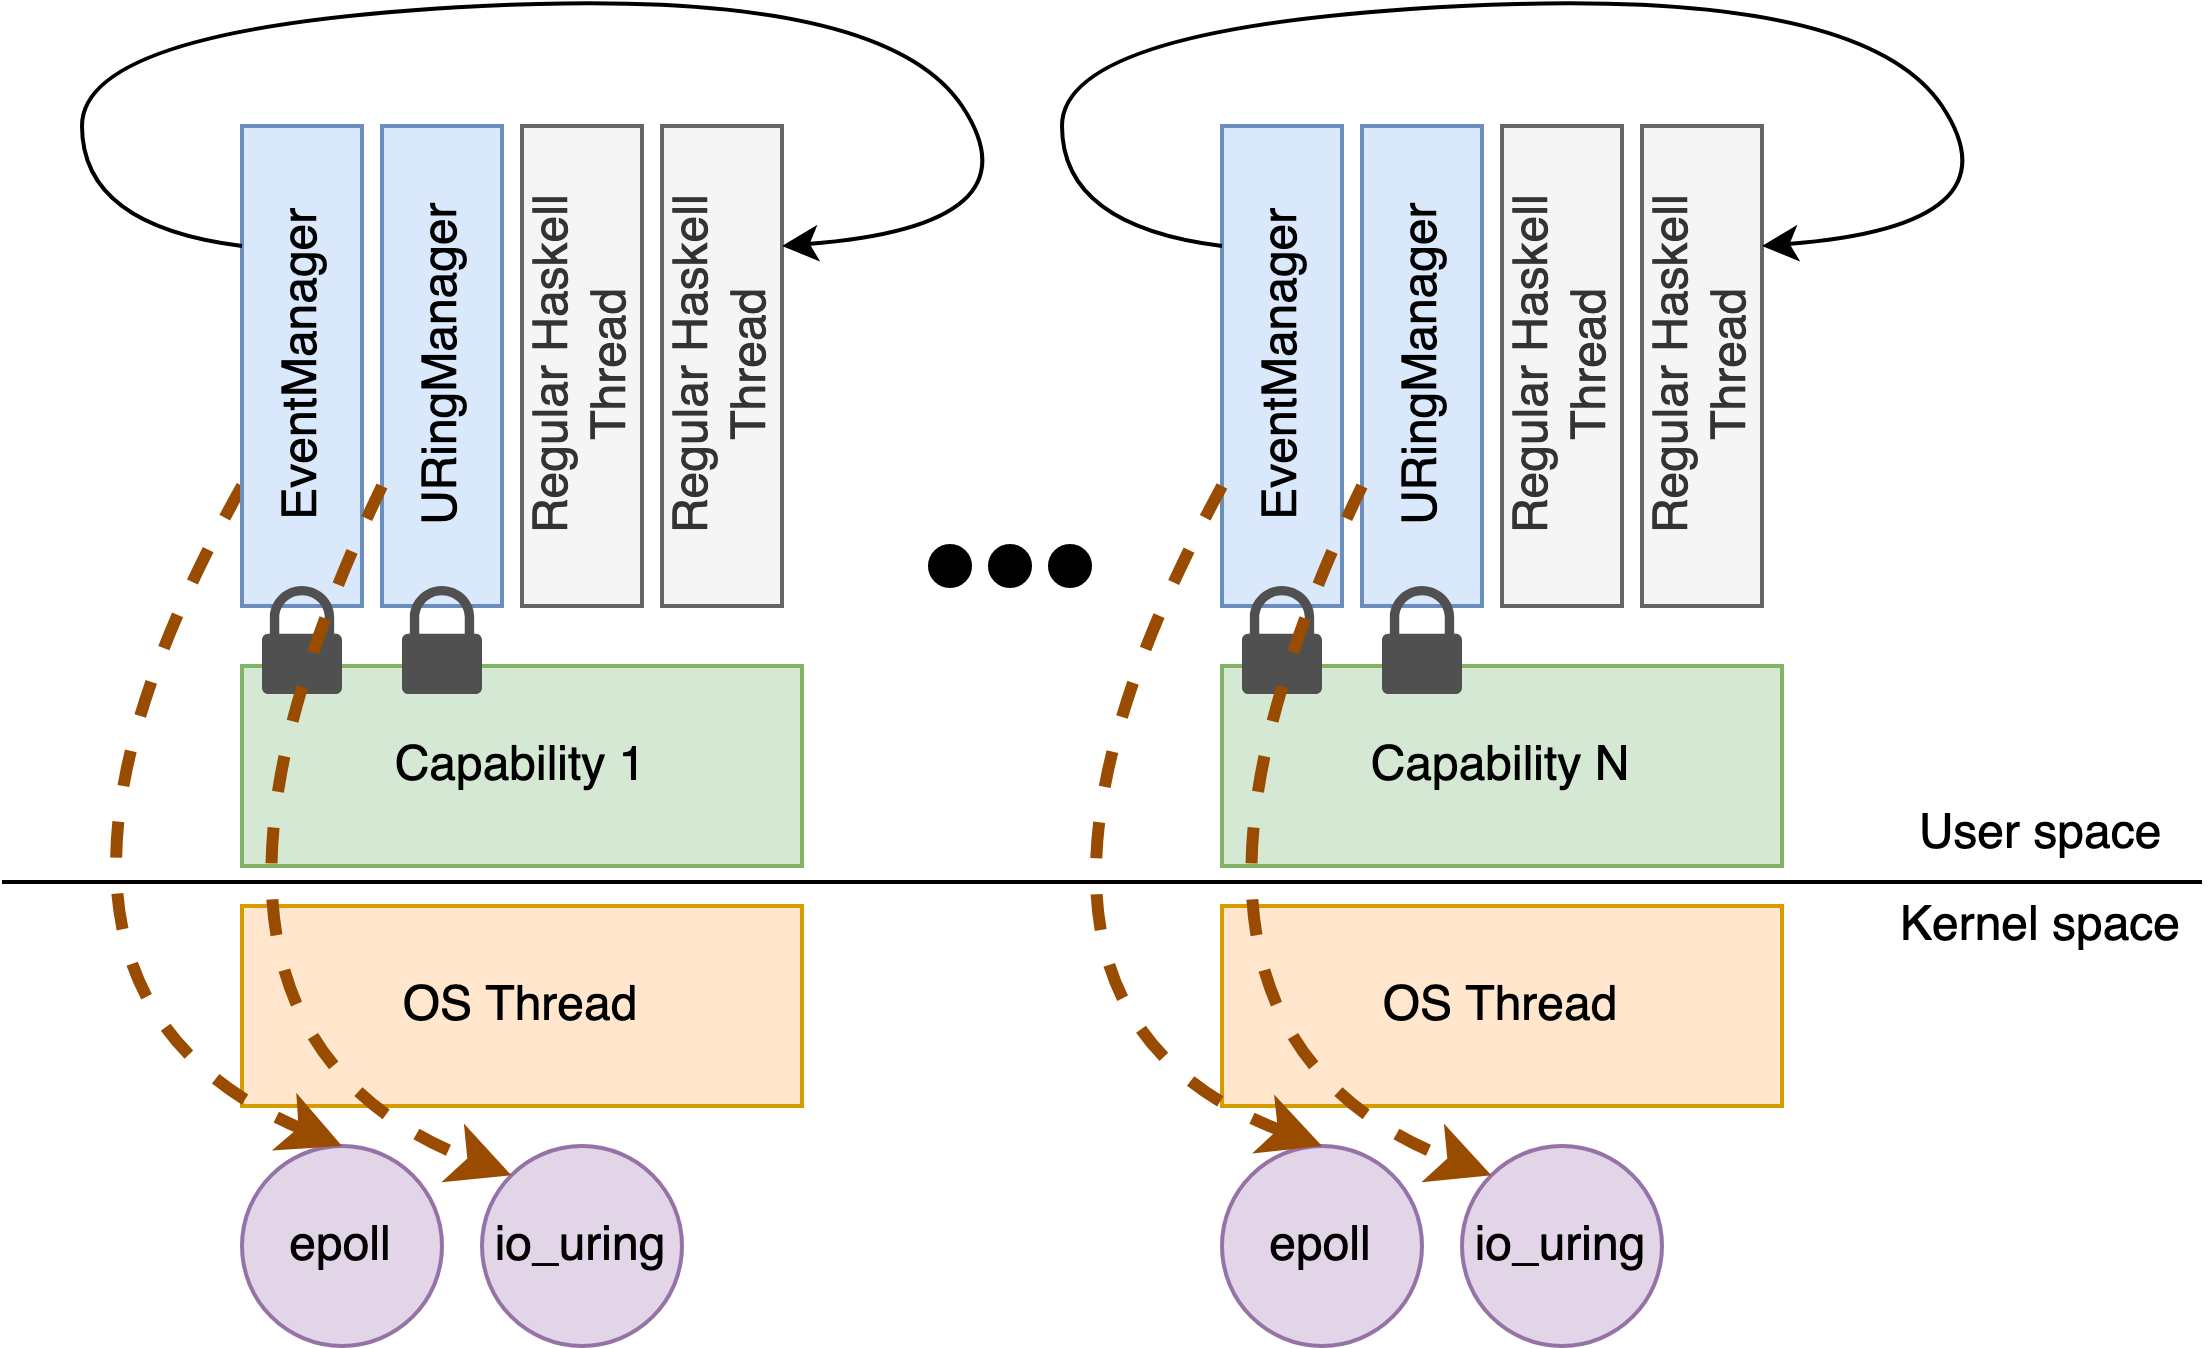
\includegraphics[width=0.85\textwidth]{figures/graphics/ghc_illustrated.png}
	\caption[Big Picture: Capability, \texttt{URingManager}, and \texttt{EventManager}]{
		Illustration of how Capabilities, \texttt{URingManager}, and \texttt{EventManager}
		fit in together in the GHC RTS.
	}
	\label{fig:ghc_illustrated}
\end{figure} 


For each Capability, we create a corresponding Capability-local \texttt{URingManager} value, and spawn a corresponding Capability-bound thread that polls for and handles new completions in a loop. Thus, the number of \texttt{io\_uring} file descriptors open is equal to the number of Capabilities set by the user. Associating each Capability with a \texttt{URingManager} and polling loop was directly inspired by each Capability having an \texttt{EventManager} and polling loop too. Refer to Figure \ref{fig:ghc_illustrated} for an illustration of how the Capability, \texttt{URingManager}, and \texttt{EventManager} fit into the GHC RTS. 


\section{Other Potential Approaches}

We alternatively considered the approach of extending the \texttt{EventManager} to become an asynchronous system call facility. In this scenario, we would extend the \texttt{EventManager} interface to include asynchronous system calls such as read and write. Registering a file descriptor can be seen as another supported system call. For the existing polling-based \texttt{EventManager} backends, implementing the asynchronous write syscall for example would involve first registering the file descriptor for writes, and then actually executing the write system call when the file descriptor is known to not block.

There were two main potential benefits from such a design. Firstly, a generalized \texttt{EventManager} would be less ad-hoc than having a separate \texttt{URingManager} interface that libraries have to conditionally depend on if the operating system is a recent-enough version of Linux. Secondly, although not tested, the \texttt{URingManager} would have to run in an additional Haskell thread, meaning potentially larger overhead.

Nevertheless, we ultimately decided against this unifying design for the following reasons. It would be hard for the unifying design to cover all possible implementation-specific requirements that other programs may have. Furthermore, it would have a higher maintenance burden for RTS maintainers to cover the addition of new system calls and implementation changes over all operating systems. Finally, the additional Haskell thread is not a concern as these threads are lightweight, and it is possible to disable either the \texttt{EventManager} or \texttt{URingManager} threads in the program if not used.
